%% ma: L10-B24-0003
%% lop: 10
%% chuong: 8
%% bai: 24
%% dang: 10.24.1
%% loai: TLN
%% muc: VD
%% dap_an: "32"
%% nguon: "(NBV)-ĐỀ SỐ 10-MỖI NGÀY 1 ĐỀ THI 2025.pdf (D10, MỖI NGÀY 1 ĐỀ - Đề số 10), Phần III Câu 2"
%% kien_thuc: "Bài 24 (chu trình qua đủ các đỉnh, đếm cách đi)"
%% trang_thai: chinh-thuc
%% ghi_chu: "Cùng ý tưởng với L10-B24-0001, L10-B24-0002 (chu trình ngắn nhất qua các đỉnh của đồ thị có trọng số), nhập vào dạng 10.24.1 đã duyệt. Đồ thị này chỉ có một chu trình qua đủ 6 đỉnh (kiểm bằng Python), đáp án 32 khớp đáp án gốc."
\begin{ex}
Giả sử có sáu địa điểm $A,B,C,D,E,F$ được nối với nhau theo những con số với độ dài (đơn vị: kilômét) được mô tả như hình bên. Một người giao hàng cần đi giao hàng tại sáu địa điểm trên. Người giao hàng xuất phát từ một địa điểm nào đó, đi qua các điểm còn lại để giao hàng, mỗi địa điểm đúng một lần và trở về địa điểm ban đầu. Quãng đường ngắn nhất mà người giao hàng có thể di chuyển là bao nhiêu kilômét?
\begin{center}
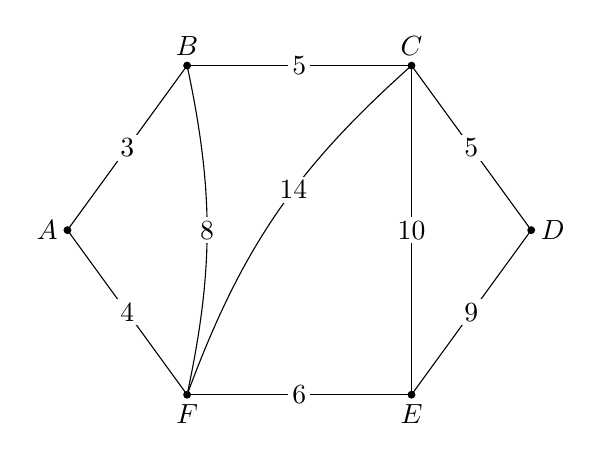
\begin{tikzpicture}[scale=.95]
  \path (0,0) coordinate (A) (1.6,2.2) coordinate (B) (4.6,2.2) coordinate (C) (6.2,0) coordinate (D) (4.6,-2.2) coordinate (E) (1.6,-2.2) coordinate (F);
  \draw (A)--(B) node[midway,fill=white,inner sep=1.5pt]{$3$};
  \draw (B)--(C) node[midway,fill=white,inner sep=1.5pt]{$5$};
  \draw (C)--(D) node[midway,fill=white,inner sep=1.5pt]{$5$};
  \draw (D)--(E) node[midway,fill=white,inner sep=1.5pt]{$9$};
  \draw (E)--(F) node[midway,fill=white,inner sep=1.5pt]{$6$};
  \draw (F)--(A) node[midway,fill=white,inner sep=1.5pt]{$4$};
  \draw (B) to[bend left=12] node[midway,fill=white,inner sep=1.5pt]{$8$} (F);
  \draw (C) to[bend right=14] node[pos=.42,fill=white,inner sep=1.5pt]{$14$} (F);
  \draw (C)--(E) node[midway,fill=white,inner sep=1.5pt]{$10$};
  \foreach \P in {A,B,C,D,E,F} \fill (\P) circle (1.5pt);
  \path (A) node[left]{$A$} (B) node[above]{$B$} (C) node[above]{$C$} (D) node[right]{$D$} (E) node[below]{$E$} (F) node[below]{$F$};
\end{tikzpicture}
\end{center}
\shortans{32}
\loigiai{Đường đi cần tìm là chu trình qua cả $6$ đỉnh, mỗi đỉnh có đúng hai cạnh của chu trình đi qua. Đỉnh $A$ chỉ nối với $B$, $F$ nên chu trình chứa $AB$, $AF$; đỉnh $D$ chỉ nối với $C$, $E$ nên chứa $DC$, $DE$. Cạnh $BF$ bị loại (sẽ khép kín tam giác $ABF$). Khi đó $B$ phải nối thêm với $C$, và $F$ nối thêm với $E$ (cạnh $FC$ bị loại vì $C$ đã có $CB$, $CD$).

Chu trình duy nhất là $A\to B\to C\to D\to E\to F\to A$ với độ dài $3+5+5+9+6+4=32$ (km).}
\end{ex}
